%%%%%%%%%%%%%%%%%%%%%%%%%%%%%%%%%%%%%%%%%%%%%%%%%%%%%%%%%%%%%%%%%%%%%%%%%%%%%%%
\section{Test Cases}
\label{sec:Test Cases}
%%%%%%%%%%%%%%%%%%%%%%%%%%%%%%%%%%%%%%%%%%%%%%%%%%%%%%%%%%%%%%%%%%%%%%%%%%%%%%%

-Benchmarks for Evaluation and Validation of Reactor Simulations (BEAVRS)~\cite{horelik2013beavrs}

-need to describe both pinwise fissoin rates and U-238 capture rates
  -latter papers can cite this one as reason to only analyze capture rates?


%%%%%%%%%%%%%%%%%%%%%%%%%%%%%%%%%%%%%%%%%%%%%%%%%%%%%%%%%%%%%%%%%%%%%%%%%%%%%%%
\subsection{Benchmark Configurations}
\label{subsec:benchmarks}

\begin{figure}[h!]
\centering
\begin{subfigure}{0.35\textwidth}
  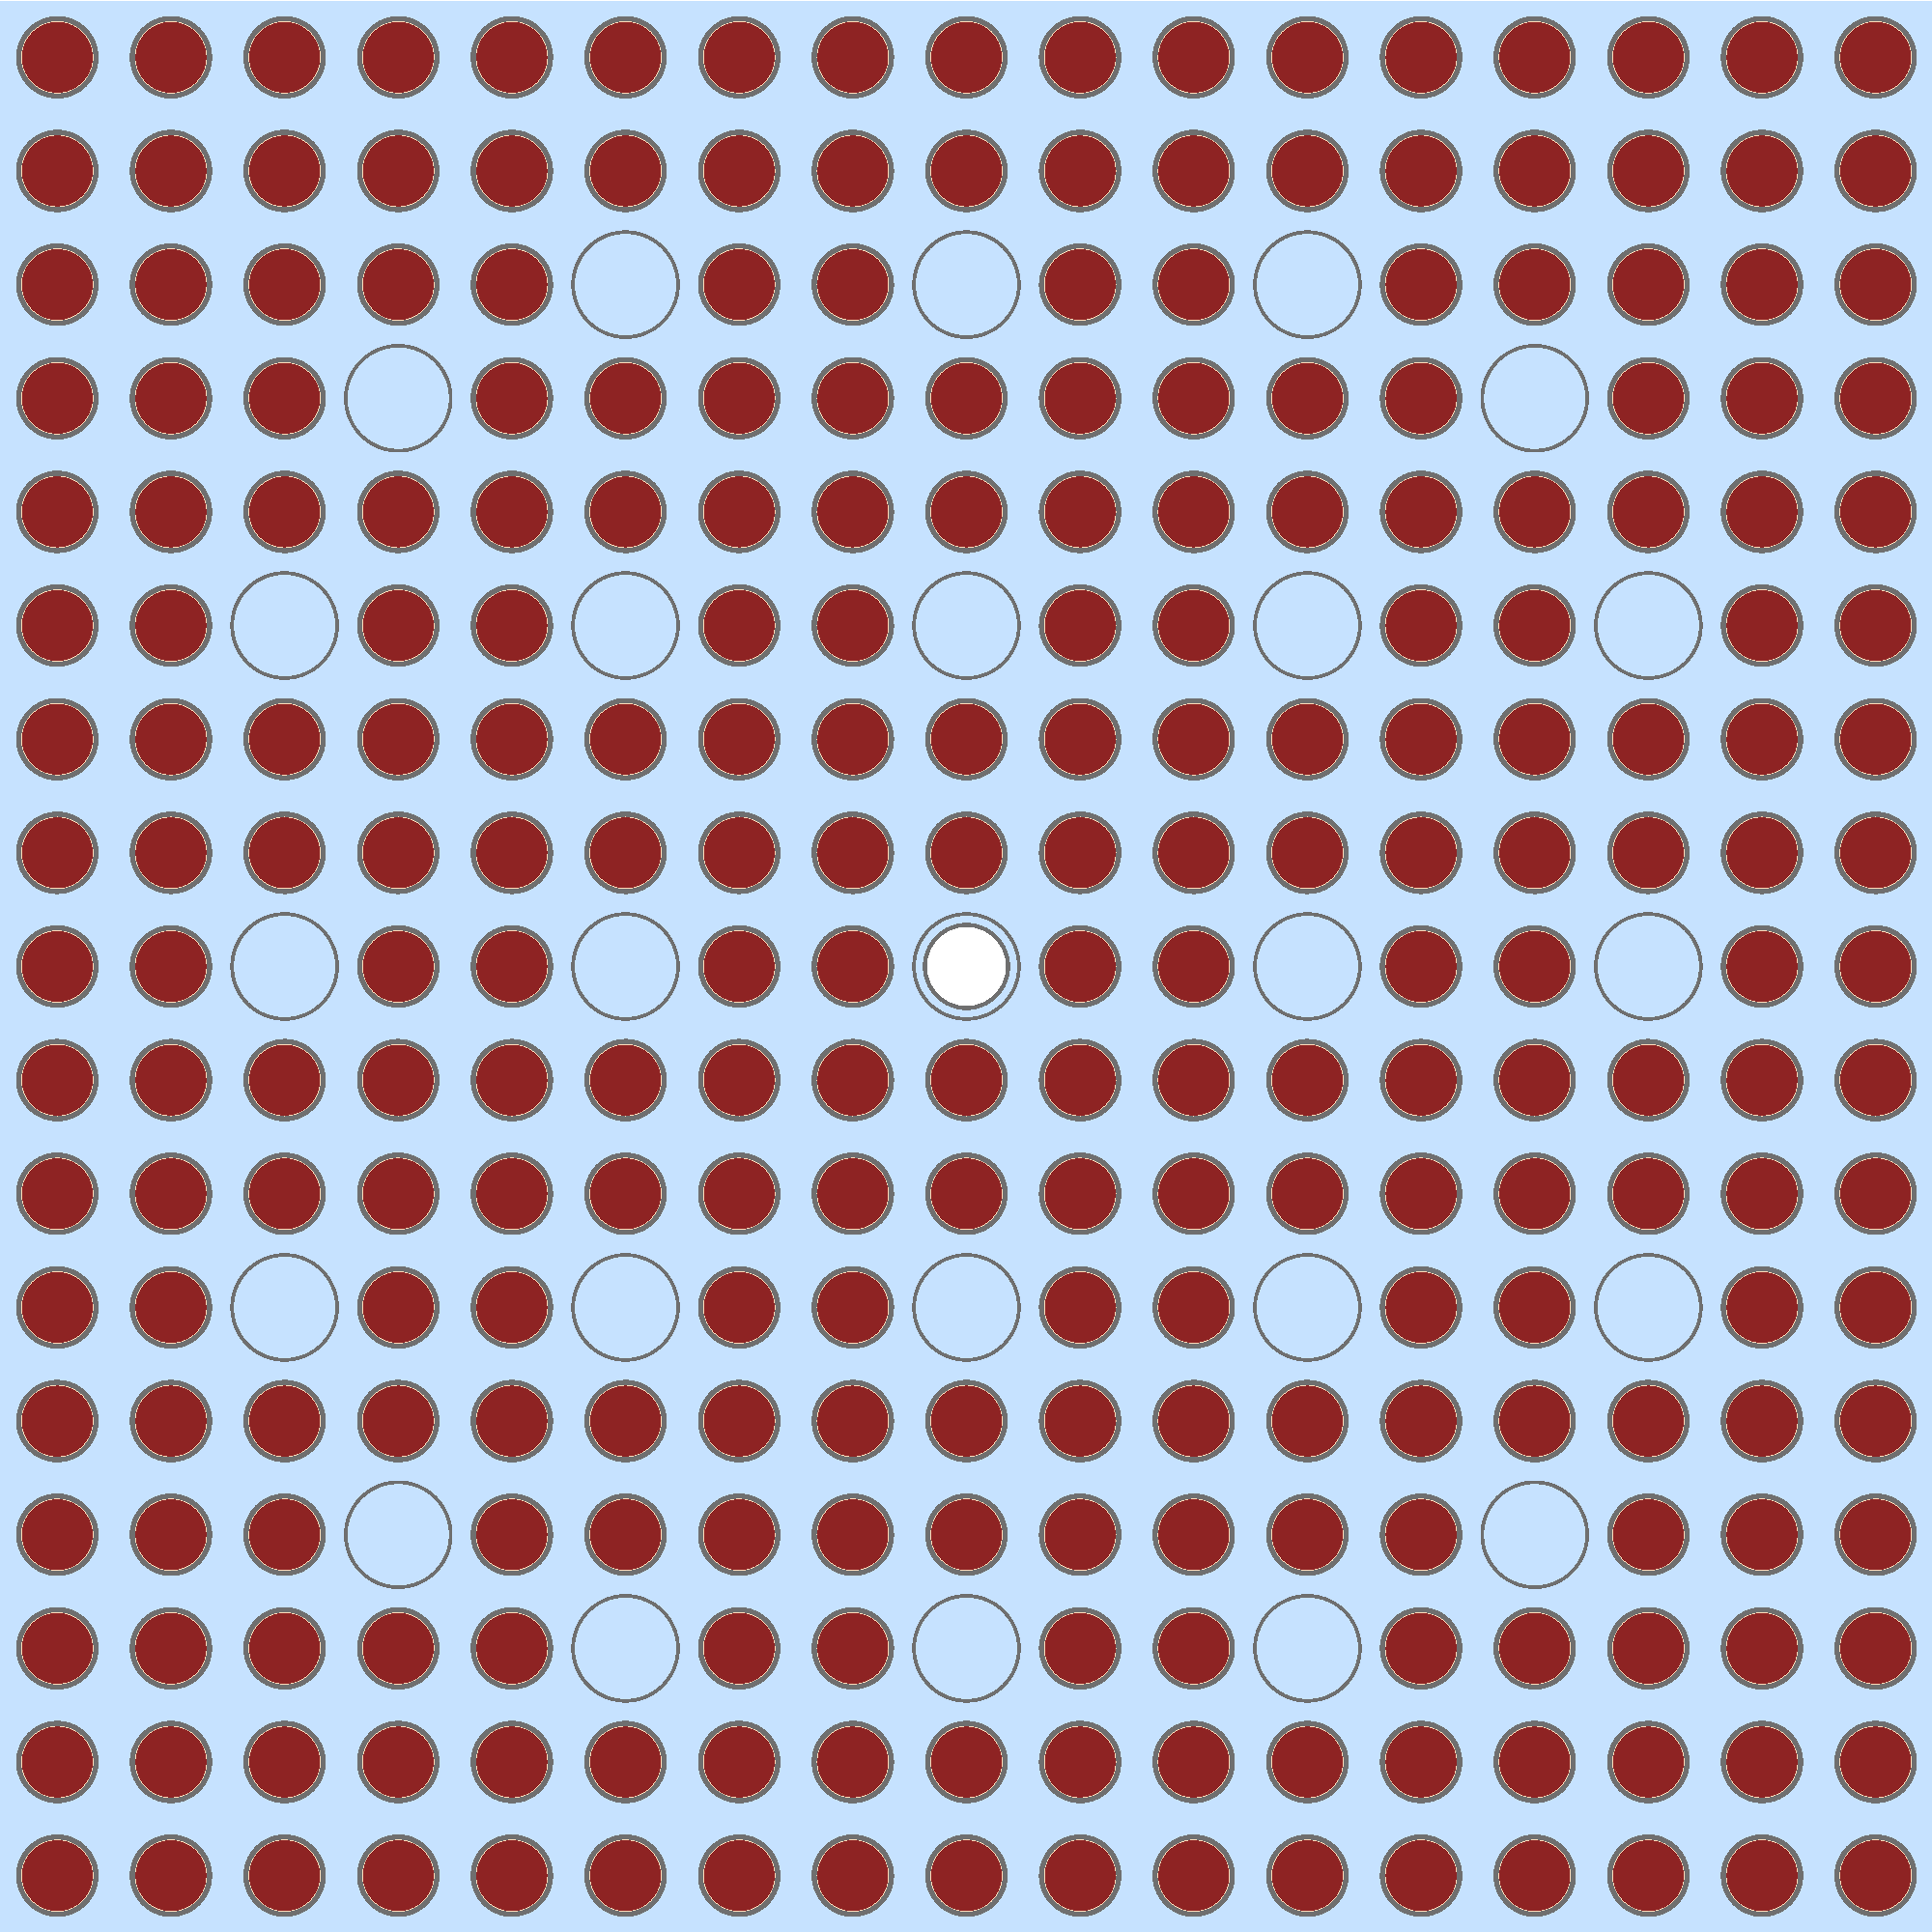
\includegraphics[width=\linewidth]{figures/assembly}
  \caption{}
  \label{fig:benchmarks-assm}
\end{subfigure}
\begin{subfigure}{0.35\textwidth}
  \centering
  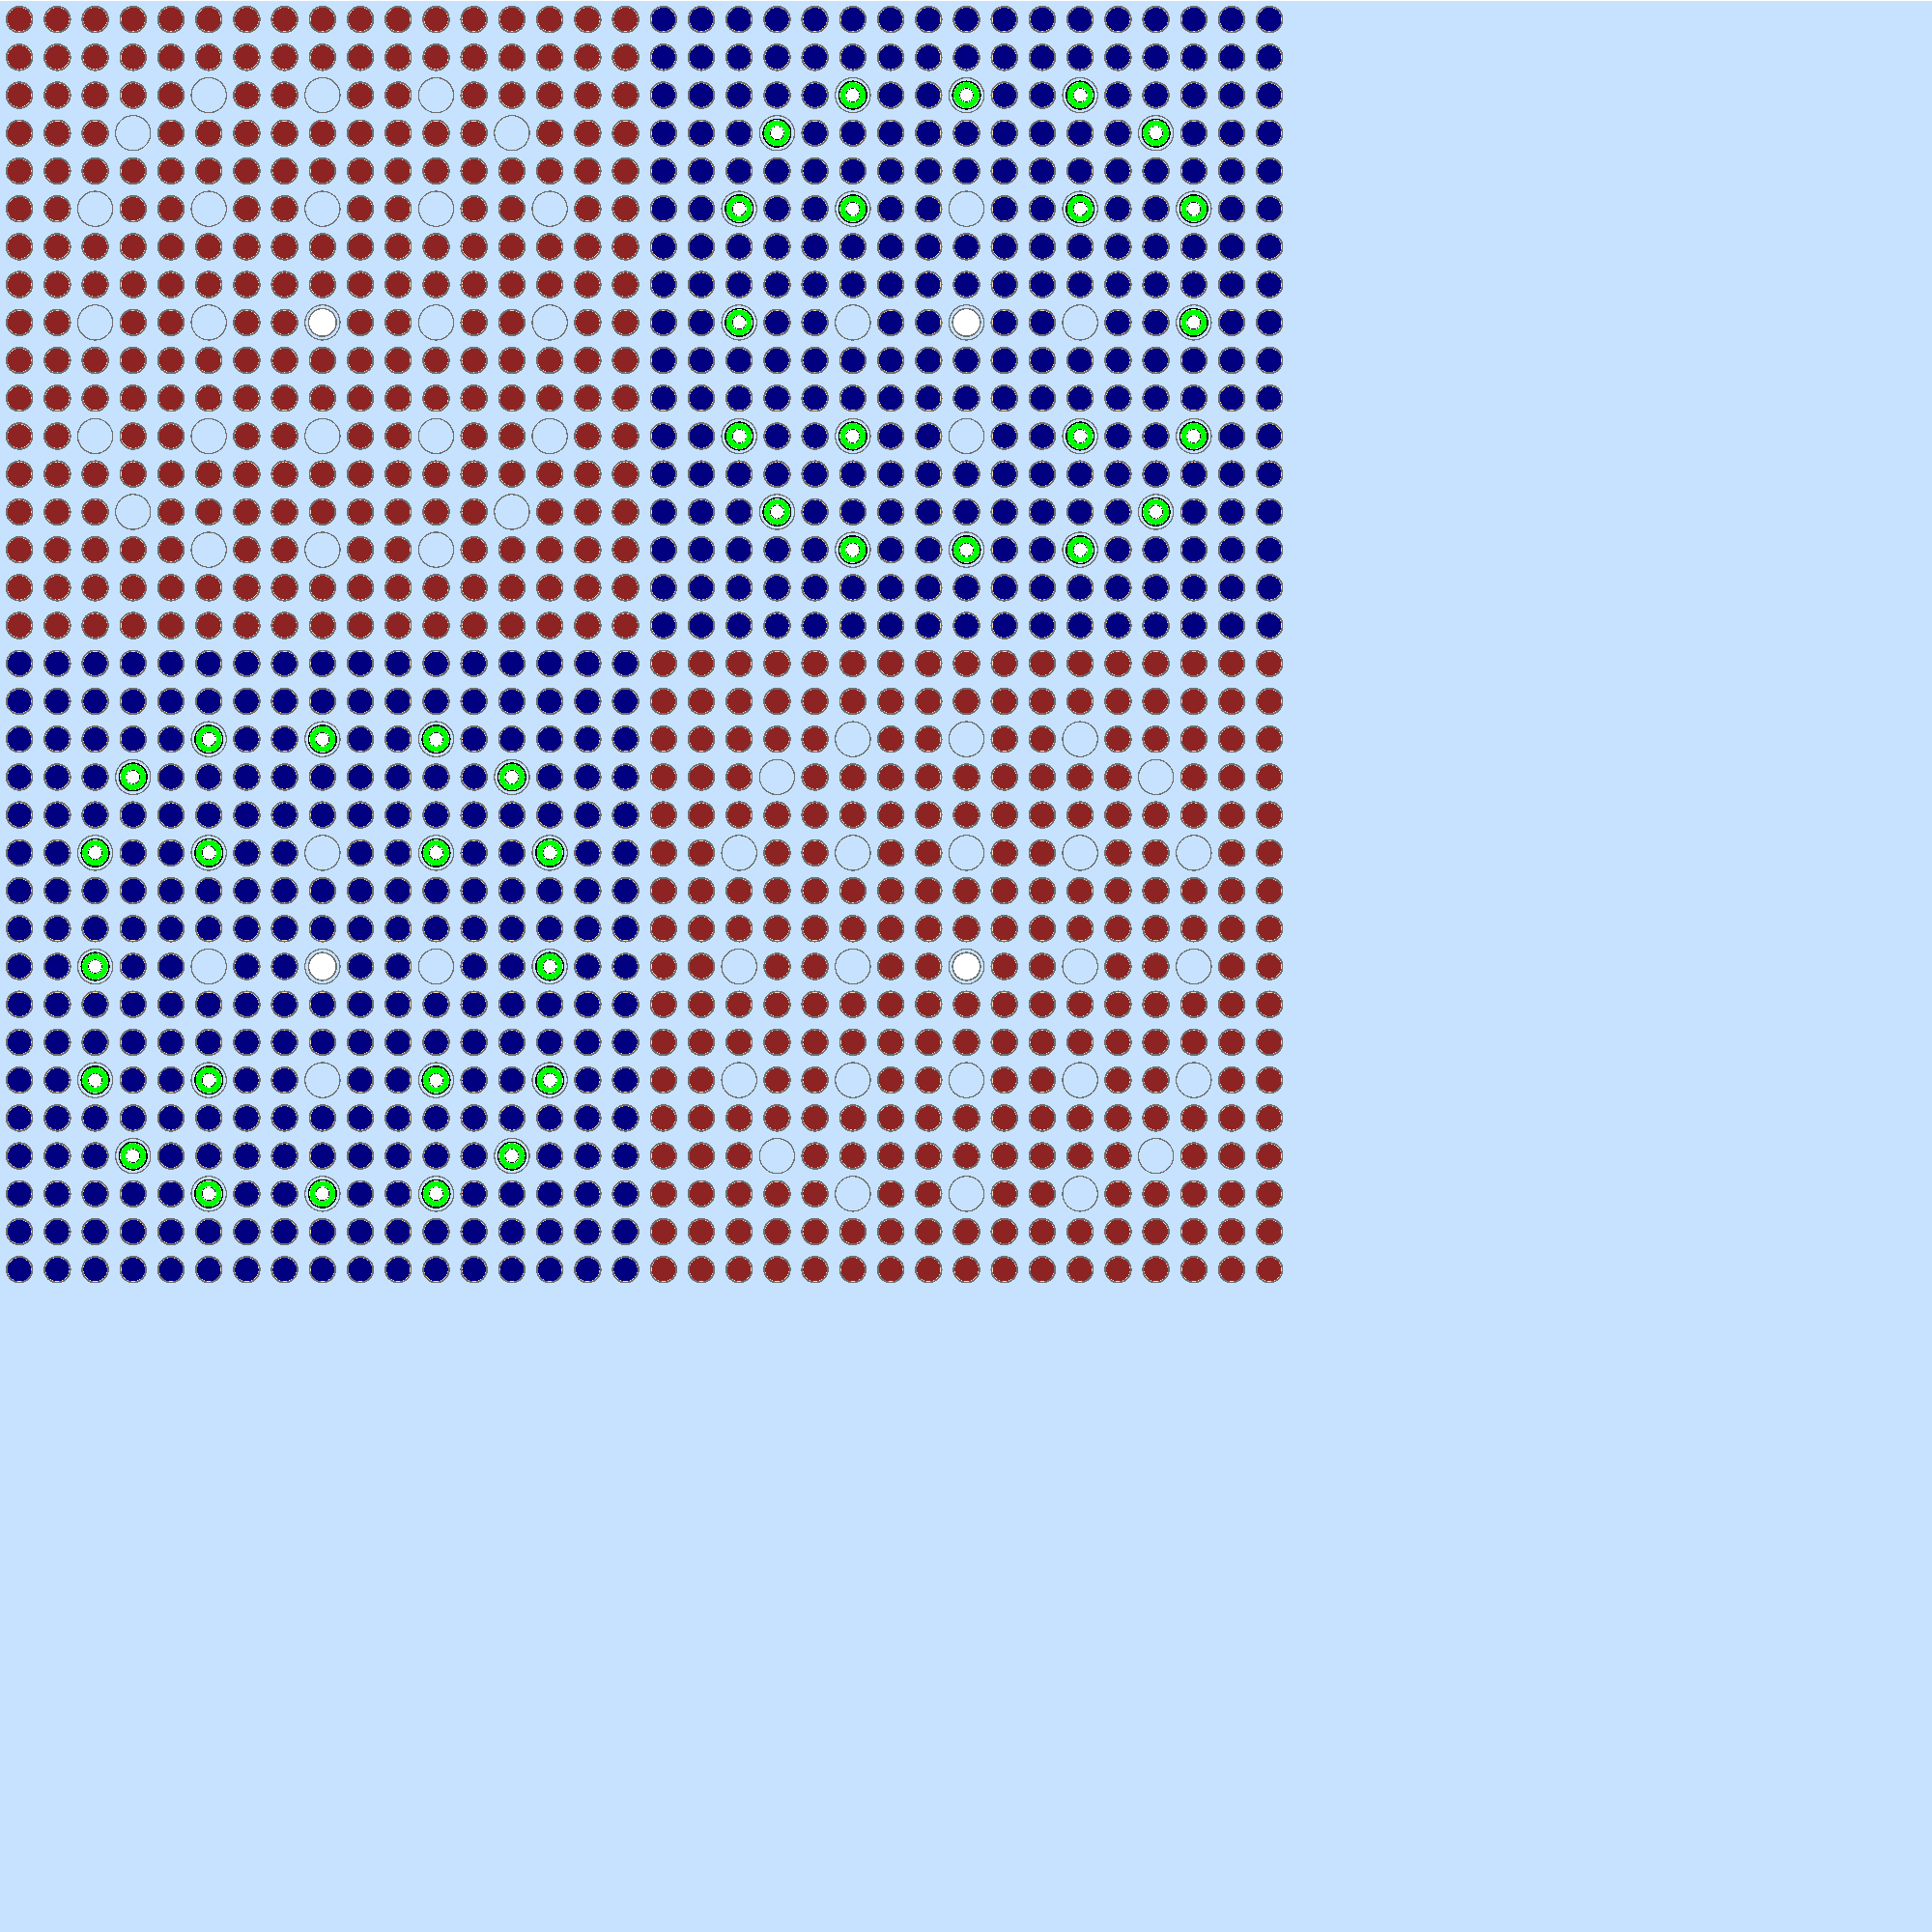
\includegraphics[width=\linewidth]{figures/reflector}
  \caption{}
  \label{fig:benchmarks-reflector}
\end{subfigure}
\caption{A (a) fuel assembly and (b) 2$\times$2 assembly colorset with reflector.}
\label{fig:benchmarks}
\end{figure}


%%%%%%%%%%%%%%%%%%%%%%%%%%%%%%%%%%%%%%%%%%%%%%%%%%%%%%%%%%%%%%%%%%%%%%%%%%%%%%%
\subsection{Single Fuel Assembly}
\label{subsubsec:benchmarks-assm}

%%%%%%%%%%%%%%%%%%%%%%%%%%%%%%%%%%%%%%%%%%%%%%%%%%%%%%%%%%%%%%%%%%%%%%%%%%%%%%%
\subsection{Reflected Assembly Colorset}
\label{subsubsec:benchmarks-2x2}



%%%%%%%%%%%%%%%%%%%%%%%%%%%%%%%%%%%%%%%%%%%%%%%%%%%%%%%%%%%%%%%%%%%%%%%%%%%%%%%
\subsection{Verification Metrics}
\label{subsec:metrics}

-reference results generated with OpenMC simulations (Sec. 7.3)
-eigenvalues
-pin-wise fission rates
-pin-wise U-238 capture rates

\begin{figure}[h!]
\centering
\begin{subfigure}{0.35\textwidth}
  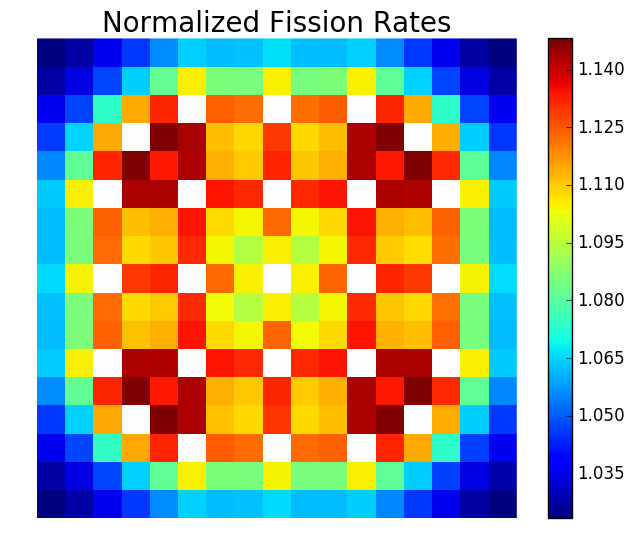
\includegraphics[width=\linewidth]{figures/fiss-assm}
  \caption{}
  \label{fig:fiss-assm}
\end{subfigure}
\begin{subfigure}{0.35\textwidth}
  \centering
  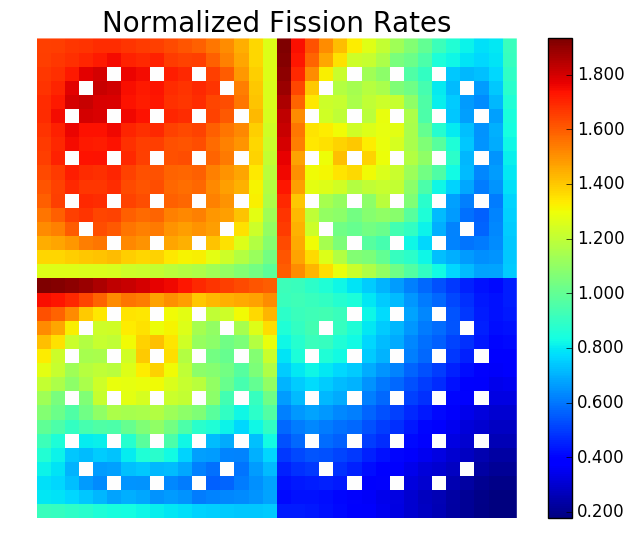
\includegraphics[width=\linewidth]{figures/fiss-reflector}
  \caption{}
  \label{fig:fiss-reflector}
\end{subfigure}
\caption{Fission rates for the (a) assembly and (b) 2$\times$2 colorset.}
\label{fig:fiss-rates}
\end{figure}

\begin{figure}[h!]
\centering
\begin{subfigure}{0.35\textwidth}
  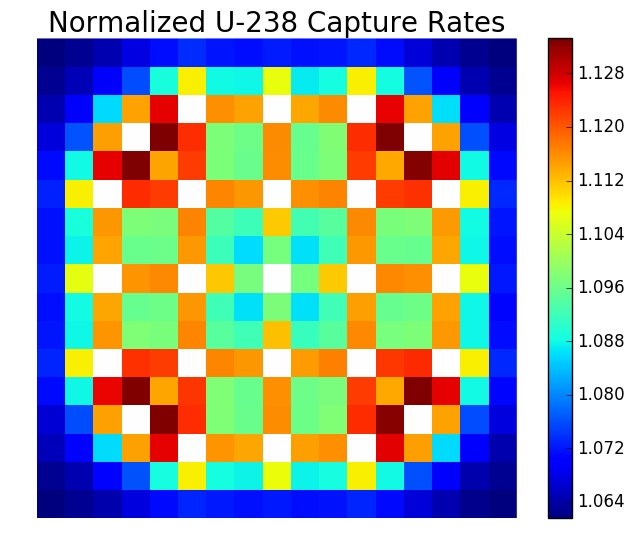
\includegraphics[width=\linewidth]{figures/capt-assm}
  \caption{}
  \label{fig:capt-assm}
\end{subfigure}
\begin{subfigure}{0.35\textwidth}
  \centering
  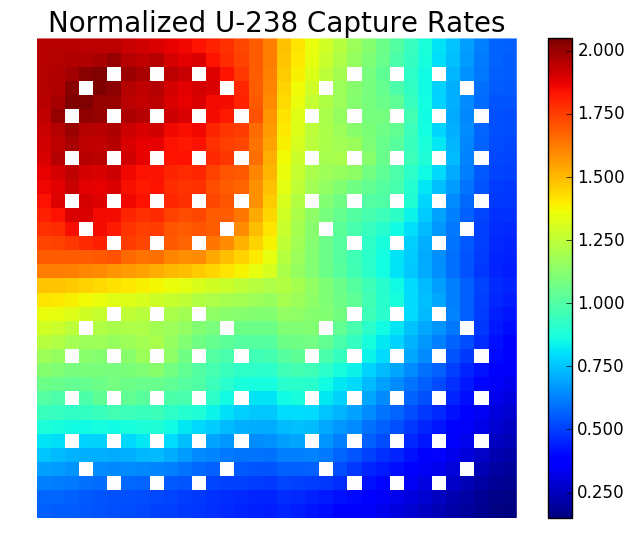
\includegraphics[width=\linewidth]{figures/capt-reflector}
  \caption{}
  \label{fig:capt-reflector}
\end{subfigure}
\caption{Capture rates for the (a) assembly and (b) 2$\times$2 colorset.}
\label{fig:capt-rates}
\end{figure}
